\documentclass[12pt]{article}
\usepackage{amsfonts,amssymb,float,amsmath}
\usepackage{algorithmic}
\usepackage{graphicx, siunintx}
\usepackage{textcomp}
\usepackage{xcolor}
\usepackage{txfonts}
\usepackage{multicol}
\usepackage{listings}
\usepackage{enumitem}
\usepackage{mathtools}
\usepackage{gensymb}
\usepackage{comment}
\usepackage[breaklinks=true]{hyperref}
\usepackage{tkz-euclide} 
\usepackage{listings}
\usepackage{gvv}                       
\usepackage{gvv-book}
%\def\inputGnumericTable{}                             
\usepackage{color}                                            
\usepackage{array}                                            
\usepackage{longtable}                                       
\usepackage{calc}                                             
\usepackage{multirow}                                         
\usepackage{hhline}                                           
\usepackage{ifthen}                                           
\usepackage{lscape}
\newcommand{\BEQA}{\begin{eqnarray}}
\newcommand{\EEQA}{\end{eqnarray}}
%\newcommand{\define}{\stackrel{\triangle}{=}}
\theoremstyle{remark}
\newtheorem{rem}{Remark}
\parindent 0px
\pagenumbering{gobble}
\begin{document}
\title{\vspace{-5cm}GATE Paper 2010 EE}
\author{Electrical Engineering}
\date{2010}
\maketitle

\begin{flushleft}
\textbf{Q.1 - Q.25 carry one mark each.}
\end{flushleft}
\begin{enumerate}
%Q.1
\item The value of the quantity P, where $P=\int_{0}^{1}xe^{x}dx,$ is equal to
\begin{enumerate}
    \begin{multicols}{4}
        \item 0
        \item 1
        \item e
        \item 1/e
    \end{multicols}
\end{enumerate}
\hfill\brak{GATE \ EE \ 2010}

%Q.2
\item Divergence of the three-dimensional radial vector field $\vec{r}$ is
\begin{enumerate}
    \begin{multicols}{4}
        \item 3
        \item $1/r$
        \item $\hat{i}+\hat{j}+\hat{k}$
        \item $3\brak{\hat{i}+\hat{j}+\hat{k}}$
    \end{multicols}
\end{enumerate}
\hfill\brak{GATE \ EE \ 2010}

%Q.3
\item The period of the signal $x\brak{t}=8\sin\brak{0.8\pi t+\frac{\pi}{4}}$ is
\begin{enumerate}
    \begin{multicols}{4}
        \item 0.4$\pi$ s
        \item 0.8$\pi$ s
        \item 1.25 s
        \item 2.5 s
    \end{multicols}
\end{enumerate}
\hfill\brak{GATE \ EE \ 2010}

%Q.4
\item The system represented by the input-output relationship $y\brak{t}=\int_{-\infty}^{5t}x\brak{\tau}d\tau, t>0$ is
\begin{enumerate}
    \begin{multicols}{2}
        \item Linear and causal
        \item Linear but not causal
        \item Causal but not linear
        \item Neither linear nor causal
    \end{multicols}
\end{enumerate}
\hfill\brak{GATE \ EE \ 2010}

%Q.5
\item The switch in the circuit has been closed for a long time. It is opened at $t=0$. At $t=0^{+}$, the current through the 1 µF capacitor is
\begin{figure}[H]
    \centering
    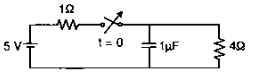
\includegraphics[width=0.4\textwidth]{Figs/Q5.png}
    \caption{}
    \label{fig:1.1}
\end{figure}
\begin{enumerate}
    \begin{multicols}{4}
        \item 0 A
        \item 1 A
        \item 1.25 A
        \item 5 A
    \end{multicols}
\end{enumerate}
\hfill\brak{GATE \ EE \ 2010}

%Q.6
\item The second harmonic component of the periodic waveform given in the figure has an amplitude of
\begin{figure}[H]
    \centering
    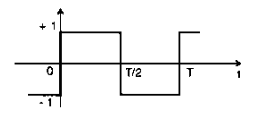
\includegraphics[width=0.4\textwidth]{Figs/Q6.png}
    \caption{}
    \label{fig:1.2}
\end{figure}
\begin{enumerate}
    \begin{multicols}{4}
        \item 0
        \item 1
        \item $2/\pi$
        \item $\sqrt{5}$
    \end{multicols}
\end{enumerate}
\hfill\brak{GATE \ EE \ 2010}

%Q.7
\item As shown in the figure, a 1$\Omega$ resistance is connected across a source that has a load line $v+i=100$. The current through the resistance is
\begin{figure}[H]
    \centering
    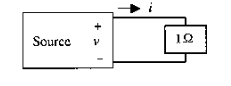
\includegraphics[width=0.3\textwidth]{Figs/Q7.png}
    \caption{}
    \label{fig:1.3}
\end{figure}
\begin{enumerate}
    \begin{multicols}{4}
        \item 25 A
        \item 50 A
        \item 100 A
        \item 200 A
    \end{multicols}
\end{enumerate}
\hfill\brak{GATE \ EE \ 2010}

%Q.8
\item A wattmeter is connected as shown in the figure. The wattmeter reads
\begin{figure}[H]
    \centering
    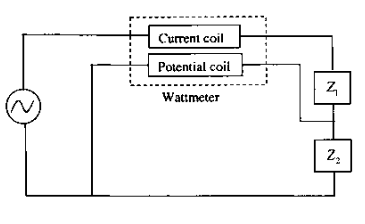
\includegraphics[width=0.6\textwidth]{Figs/Q8.png}
    \caption{}
    \label{fig:1.4}
\end{figure}
\begin{enumerate}
    \item Zero always
    \item Total power consumed by $Z_1$ and $Z_2$
    \item Power consumed by $Z_1$
    \item Power consumed by $Z_2$
\end{enumerate}
\hfill\brak{GATE \ EE \ 2010}

%Q.9
\item An ammeter has a current range of 0-5 A, and its internal resistance is 0.2 $\Omega$. In order to change the range to 0-25 A, we need to add a resistance of
\begin{enumerate}
    \item 0.8 $\Omega$ in series with the meter.
    \item 1.0 $\Omega$ in series with the meter.
    \item 0.04 $\Omega$ in parallel with the meter.
    \item 0.05 $\Omega$ in parallel with the meter.
\end{enumerate}
\hfill\brak{GATE \ EE \ 2010}

%Q.10
\item As shown in the figure, a negative feedback system has an amplifier of gain 100 with $\pm10\%$ tolerance in the forward path, and an attenuator of value $9/100$ in the feedback path. The overall system gain is approximately:
\begin{figure}[H]
    \centering
    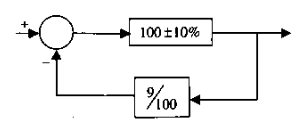
\includegraphics[width=0.5\textwidth]{Figs/Q10.png}
    \caption{}
    \label{fig:1.5}
\end{figure}
\begin{enumerate}
    \begin{multicols}{2}
        \item $10\pm1\%$
        \item $10\pm2\%$
        \item $10\pm5\%$
        \item $10\pm10\%$
    \end{multicols}
\end{enumerate}
\hfill\brak{GATE \ EE \ 2010}

%Q.11
\item For the system $\frac{2}{\brak{s+1}}$, the approximate time taken for a step response to reach 98\% of its final value is
\begin{enumerate}
    \begin{multicols}{4}
        \item 1s
        \item 2s
        \item 4s
        \item 8s
    \end{multicols}
\end{enumerate}
\hfill\brak{GATE \ EE \ 2010}

%Q.12
\item If the electrical circuit of figure \brak{b} is an equivalent of the coupled tank system of figure \brak{a}, then
\begin{figure}[H]
    \centering
    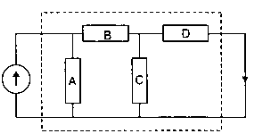
\includegraphics[width=0.8\textwidth]{Figs/Q12.png}
    \caption{}
    \label{fig:1.6}
\end{figure}
\begin{enumerate}
    \item A, B are resistances and C, D capacitances
    \item A, C are resistances and B, D capacitances
    \item A, B are capacitances and C, D resistances
    \item A, C are capacitances and B, D resistances
\end{enumerate}
\hfill\brak{GATE \ EE \ 2010}

%Q.13
\item A single-phase transformer has a turns ratio of 1:2, and is connected to a purely resistive load as shown in the figure. The magnetizing current drawn is 1 A, and the secondary current is 1 A. If core losses and leakage reactances are neglected, the primary current is
\begin{figure}[H]
    \centering
    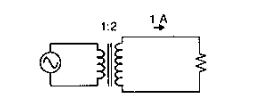
\includegraphics[width=0.4\textwidth]{Figs/Q13.png}
    \caption{}
    \label{fig:1.7}
\end{figure}
\begin{enumerate}
    \begin{multicols}{4}
        \item 1.41 A
        \item 2 A
        \item 2.24 A
        \item 3 A
    \end{multicols}
\end{enumerate}
\hfill\brak{GATE \ EE \ 2010}

%Q.14
\item Power is transferred from system A to system B by an HVDC link as shown in the figure. If the voltages $V_{AB}$ and $V_{CD}$ are as indicated in the figure, and $i>0$, then
\begin{figure}[H]
    \centering
    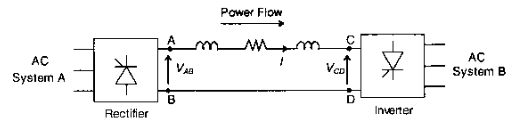
\includegraphics[width=0.8\textwidth]{Figs/Q14.png}
    \caption{}
    \label{fig:1.8}
\end{figure}
\begin{enumerate}
    \item $V_{AB} < 0$, $V_{CD} < 0$, $V_{AB} > V_{CD}$
    \item $V_{AB} > 0$, $V_{CD} > 0$, $V_{AB} < V_{CD}$
    \item $V_{AB} > 0$, $V_{CD} > 0$, $V_{AB} > V_{CD}$
    \item $V_{AB} > 0$, $V_{CD} < 0$
\end{enumerate}
\hfill\brak{GATE \ EE \ 2010}

%Q.15
\item A balanced three-phase voltage is applied to a star-connected induction motor, the phase to neutral voltage being V. The stator resistance, rotor resistance referred to the stator, stator leakage reactance, rotor leakage reactance referred to the stator, and the magnetizing reactance are denoted by $r_s, r_r', x_s, x_r'$ and $X_m$ respectively. The magnitude of the starting current of the motor is given by:
\begin{enumerate}
    \begin{multicols}{2}
        \item $\frac{V}{\sqrt{\brak{r_s+r_r'}^2 + \brak{x_s+x_r'}^2}}$
        \item $\frac{V}{\sqrt{r_s^2 + \brak{x_s+X_m}^2}}$
        \item $\frac{V}{\sqrt{\brak{r_s+r_r'}^2 + \brak{X_m+x_r'}^2}}$
        \item $\frac{V}{\sqrt{r_s^2 + \brak{X_m+x_s'}^2}}$
    \end{multicols}
\end{enumerate}
\hfill\brak{GATE \ EE \ 2010}

%Q.16
\item Consider a step voltage wave of magnitude 1 pu travelling along a lossless transmission line that terminates in a reactor. The voltage magnitude across the reactor at the instant the travelling wave reaches the reactor is
\begin{figure}[H]
    \centering
    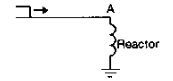
\includegraphics[width=0.25\textwidth]{Figs/Q16.png}
    \caption{}
    \label{fig:1.9}
\end{figure}
\begin{enumerate}
    \begin{multicols}{2}
        \item -1 pu
        \item 1 pu
        \item 2 pu
        \item 3 pu
    \end{multicols}
\end{enumerate}
\hfill\brak{GATE \ EE \ 2010}

%Q.17
\item Consider two buses connected by an impedance of $\brak{0+j5} \Omega$. The bus 1 voltage is $100\angle30^{\circ}$V and bus 2 voltage is $100\angle0^{\circ}$ V. The real and reactive power supplied by bus 1, respectively, are
\begin{enumerate}
    \begin{multicols}{2}
        \item 1000 W, 268 VAr
        \item -1000 W, -134 VAr
        \item 276.9 W, -56.7 VAr
        \item -276.9 W, 56.7 VAr
    \end{multicols}
\end{enumerate}
\hfill\brak{GATE \ EE \ 2010}

%Q.18
\item A three-phase, 33 kV oil circuit breaker is rated 1200 A, 2000 MVA, 3 s. The symmetrical breaking current is
\begin{enumerate}
    \begin{multicols}{2}
        \item 1200 A
        \item 3600 A
        \item 35 kA
        \item 104.8 kA
    \end{multicols}
\end{enumerate}
\hfill\brak{GATE \ EE \ 2010}

%Q.19
\item Consider a stator winding of an alternator with an internal high-resistance ground fault. The currents under the fault condition are as shown in the figure. The winding is protected using a differential current scheme with current transformers of ratio 400/5 A as shown. The current through the operating coil is
\begin{figure}[H]
    \centering
    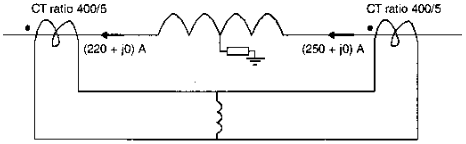
\includegraphics[width=0.9\textwidth]{Figs/Q19.png}
    \caption{}
    \label{fig:1.10}
\end{figure}
\begin{enumerate}
    \begin{multicols}{2}
        \item 0.1875 A
        \item 0.2 A
        \item 0.375 A
        \item 60 kA
    \end{multicols}
\end{enumerate}
\hfill\brak{GATE \ EE \ 2010}

%Q.20
\item The zero-sequence circuit of the three phase transformer shown in the figure is
\begin{figure}[H]
    \centering
    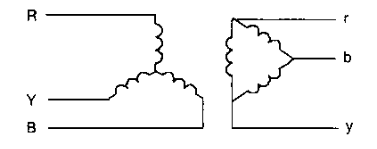
\includegraphics[width=0.7\textwidth]{Figs/Q20.png}
    \caption{}
    \label{fig:1.11}
\end{figure}
\hfill\brak{GATE \ EE \ 2010}

%Q.21
\item Given that the op-amp is ideal, the output voltage $V_0$ is
\begin{figure}[H]
    \centering
    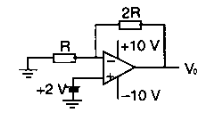
\includegraphics[width=0.4\textwidth]{Figs/Q21.png}
    \caption{}
    \label{fig:1.12}
\end{figure}
\begin{enumerate}
    \begin{multicols}{2}
        \item 4 V
        \item 6 V
        \item 7.5 V
        \item 12.12 V
    \end{multicols}
\end{enumerate}
\hfill\brak{GATE \ EE \ 2010}

%Q.22
\item Assuming that the diodes in the given circuit are ideal, the voltage $V_0$ is
\begin{figure}[H]
    \centering
    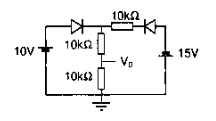
\includegraphics[width=0.5\textwidth]{Figs/Q22.png}
    \caption{}
    \label{fig:1.13}
\end{figure}
\begin{enumerate}
    \begin{multicols}{2}
        \item 4 V
        \item 5 V
        \item 7.5 V
        \item 12.12 V
    \end{multicols}
\end{enumerate}
\hfill\brak{GATE \ EE \ 2010}

%Q.23
\item The power electronic converter shown in the figure has a single-pole double-throw switch. The pole P of the switch is connected alternately to throws A and B. The converter shown is a
\begin{figure}[H]
    \centering
    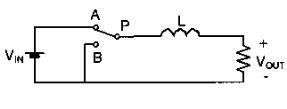
\includegraphics[width=0.5\textwidth]{Figs/Q23.png}
    \caption{}
    \label{fig:1.14}
\end{figure}
\begin{enumerate}
    \item step-down chopper \brak{buck converter}
    \item half-wave rectifier
    \item step-up chopper \brak{boost converter}
    \item full-wave rectifier
\end{enumerate}
\hfill\brak{GATE \ EE \ 2010}

%Q.24
\item Figure shows a composite switch consisting of a power transistor \brak{BJT} in series with a diode. Assuming that the transistor switch and the diode are ideal, the I-V characteristic of the composite switch is
\begin{figure}[H]
    \centering
    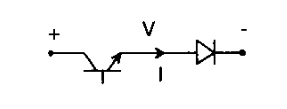
\includegraphics[width=0.25\textwidth]{Figs/Q24.png}
    \caption{Main Circuit}
    \label{fig:1.15}
\end{figure}
\begin{enumerate}
    \item \begin{figure}[H]\centering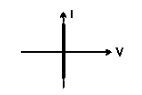
\includegraphics[width=0.4\textwidth]{Figs/Q24A.png}\caption{Option A}\label{fig:1.16}\end{figure}
    \item \begin{figure}[H]\centering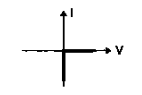
\includegraphics[width=0.4\textwidth]{Figs/Q24B.png}\caption{Option B}\label{fig:1.17}\end{figure}
    \item \begin{figure}[H]\centering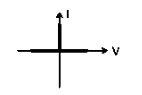
\includegraphics[width=0.4\textwidth]{Figs/Q24C.png}\caption{Option C}\label{fig:1.18}\end{figure}
    \item \begin{figure}[H]\centering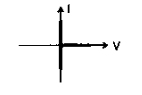
\includegraphics[width=0.4\textwidth]{Figs/Q24D.png}\caption{Option D}\label{fig:1.19}\end{figure}
\end{enumerate}
\hfill\brak{GATE \ EE \ 2010}

%Q.25
\item The fully controlled thyristor converter in the figure is fed from a single-phase source. When the firing angle is $0^{\circ}$, the dc output voltage of the converter is 300 V. What will be the output voltage for a firing angle of $60^{\circ}$, assuming continuous conduction?
\begin{figure}[H]
    \centering
    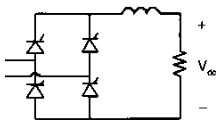
\includegraphics[width=0.4\textwidth]{Figs/Q25.png}
    \caption{}
    \label{fig:1.20}
\end{figure}
\begin{enumerate}
    \begin{multicols}{2}
        \item 150 V
        \item 210 V
        \item 300 V
        \item 100$\pi$ V
    \end{multicols}
\end{enumerate}
\hfill\brak{GATE \ EE \ 2010}

\newpage
\begin{flushleft}
\textbf{Q.26 - Q.55 carry two marks each.}
\end{flushleft}

%Q.26
\item At $t=0$, the function $f\brak{t}=\frac{\sin t}{t}$ has
\begin{enumerate}
    \begin{multicols}{2}
        \item a minimum
        \item a discontinuity
        \item a point of inflection
        \item a maximum
    \end{multicols}
\end{enumerate}
\hfill\brak{GATE \ EE \ 2010}

%Q.27
\item A box contains 4 white balls and 3 red balls. In succession, two balls are randomly selected and removed from the box. Given that the first removed ball is white, the probability that the second removed ball is red is
\begin{enumerate}
    \begin{multicols}{4}
        \item 1/3
        \item 3/7
        \item 1/2
        \item 4/7
    \end{multicols}
\end{enumerate}
\hfill\brak{GATE \ EE \ 2010}

%Q.28
\item An eigenvector of $P=\myvec{ 1 & 1 & 0 \\ 0 & 2 & 2 \\ 0 & 0 & 3}$ is
\begin{enumerate}
    \begin{multicols}{2}
        \item $\sbrak{-1 \ 1 \ 1}^T$
        \item $\sbrak{1 \ 2 \ 1}^T$
        \item $\sbrak{1 \ -1 \ 2}^T$
        \item $\sbrak{2 \ 1 \ -1}^T$
    \end{multicols}
\end{enumerate}
\hfill\brak{GATE \ EE \ 2010}

%Q.29
\item For the differential equation $\frac{d^2x}{dt^2} + 6\frac{dx}{dt} + 8x = 0$ with initial conditions $x\brak{0}=1$ and $\frac{dx}{dt}|_{t=0}=0$, the solution is
\begin{enumerate}
    \begin{multicols}{2}
        \item $x\brak{t} = 2e^{-4t} - e^{-2t}$
        \item $x\brak{t} = 2e^{-2t} - e^{-4t}$
        \item $x\brak{t} = -e^{-6t} + 2e^{-2t}$
        \item $x\brak{t} = e^{-2t} + 2e^{-4t}$
    \end{multicols}
\end{enumerate}
\hfill\brak{GATE \ EE \ 2010}

%Q.30
\item For the set of equations, $x_1 + 2x_2 + x_3 + 4x_4 = 2$, $3x_1 + 6x_2 + 3x_3 + 12x_4 = 6$, the following statement is true:
\begin{enumerate}
    \item Only the trivial solution $x_1=x_2=x_3=x_4=0$ exists.
    \item There are no solutions.
    \item A unique non-trivial solution exists.
    \item Multiple non-trivial solutions exist.
\end{enumerate}
\hfill\brak{GATE \ EE \ 2010}

%Q.31
\item $x\brak{t}$ is a positive rectangular pulse from $t=-1$ to $t=+1$ with unit height as shown in the figure. The value of $\int_{-\infty}^{\infty} |X\brak{\omega}|^2 d\omega$ where $X\brak{\omega}$ is the Fourier transform of $x\brak{t}$ is
\begin{figure}[H]
    \centering
    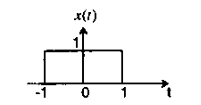
\includegraphics[width=0.3\textwidth]{Figs/Q31.png}
    \caption{}
    \label{fig:1.21}
\end{figure}
\begin{enumerate}
    \begin{multicols}{4}
        \item 2
        \item 2$\pi$
        \item 4
        \item 4$\pi$
    \end{multicols}
\end{enumerate}
\hfill\brak{GATE \ EE \ 2010}
%Q.32
\item Given the finite length input $x\sbrak{n}$ and the corresponding finite length output $y\sbrak{n}$ of an LTI system as shown below, the impulse response $h\sbrak{n}$ of the system is
\newline $x\sbrak{n}=\{1, -1\}$ (arrow at 1)
\newline $y\sbrak{n}=\{1, 0, 0, 0, -1\}$ (arrow at 1)
\begin{enumerate}
    \begin{multicols}{2}
        \item $h\sbrak{n}=\{1,0,0,1\}$
        \item $h\sbrak{n}=\{1,0,1\}$
        \item $h\sbrak{n}=\{1,1,1,1\}$
        \item $h\sbrak{n}=\{1,1,1\}$
    \end{multicols}
\end{enumerate}
\hfill\brak{GATE \ EE \ 2010}

%Q.33
\item If the 12$\Omega$ resistor draws a current of 1 A as shown in the figure, the value of resistance R is
\begin{figure}[H]
    \centering
    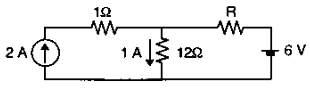
\includegraphics[width=0.5\textwidth]{Figs/Q33.png}
    \caption{}
    \label{fig:1.22}
\end{figure}
\begin{enumerate}
    \begin{multicols}{4}
        \item 4 $\Omega$
        \item 6 $\Omega$
        \item 8 $\Omega$
        \item 18 $\Omega$
    \end{multicols}
\end{enumerate}
\hfill\brak{GATE \ EE \ 2010}

%Q.34
\item The two-port network P shown in the figure has ports 1 and 2, denoted by terminals \brak{a, b} and \brak{c, d}, respectively. It has an impedance matrix Z with parameters denoted by $z_{ij}$. A 1$\Omega$ resistor is connected in series with the network at port 1 as shown in the figure. The impedance matrix of the modified two-port network \brak{shown\ as\ a\ dashed\ box} is
\begin{figure}[H]
    \centering
    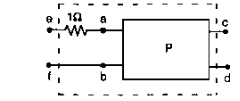
\includegraphics[width=0.5\textwidth]{Figs/Q34.png}
    \caption{}
    \label{fig:1.23}
\end{figure}
\begin{enumerate}
    \begin{multicols}{2}
        \item $\myvec{ z_{11}+1 & z_{12}+1 \\ z_{21} & z_{22}+1 }$
        \item $\myvec{ z_{11}+1 & z_{12} \\ z_{21} & z_{22}+1 }$
        \item $\myvec{ z_{11}+1 & z_{12} \\ z_{21} & z_{22} }$
        \item $\myvec{ z_{11}+1 & z_{12} \\ z_{21}+1 & z_{22} }$
    \end{multicols}
\end{enumerate}
\hfill\brak{GATE \ EE \ 2010}

%Q.35
\item The Maxwell's bridge shown in the figure is at balance. The parameters of the inductive coil are
\begin{figure}[H]
    \centering
    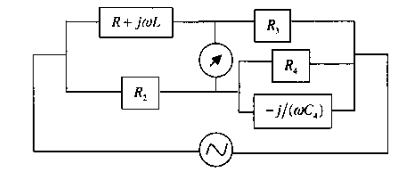
\includegraphics[width=0.7\textwidth]{Figs/Q35.png}
    \caption{}
    \label{fig:1.24}
\end{figure}
\begin{enumerate}
    \item $R=\frac{R_2 R_3}{R_4}$, $L=C_4 R_2 R_3$
    \item $L=\frac{R_2 R_3}{R_4}$, $R=C_4 R_2 R_3$
    \item $R=\frac{R_4}{R_2 R_3}$, $L=\frac{1}{C_4 R_2 R_3}$
    \item $L=\frac{R_4}{R_2 R_3}$, $R=\frac{1}{C_4 R_2 R_3}$
\end{enumerate}
\hfill\brak{GATE \ EE \ 2010}

%Q.36
\item The frequency response of $G\brak{s}=1/\sbrak{s\brak{s+1}\brak{s+2}}$ plotted in the complex $G\brak{j\omega}$ plane \brak{for\ 0 < \omega < \infty} is
\begin{enumerate}
    \item \begin{figure}[H]\centering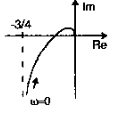
\includegraphics[width=0.4\textwidth]{Figs/Q36A.png}\caption{}\label{fig:1.25}\end{figure}
    \item \begin{figure}[H]\centering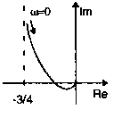
\includegraphics[width=0.4\textwidth]{Figs/Q36B.png}\caption{}\label{fig:1.26}\end{figure}
    \item \begin{figure}[H]\centering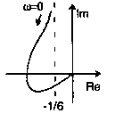
\includegraphics[width=0.4\textwidth]{Figs/Q36C.png}\caption{}\label{fig:1.27}\end{figure}
    \item \begin{figure}[H]\centering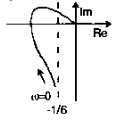
\includegraphics[width=0.4\textwidth]{Figs/Q36D.png}\caption{}\label{fig:1.28}\end{figure}
\end{enumerate}
\hfill\brak{GATE \ EE \ 2010}

%Q.37
\item The system $\dot{x}=Ax+Bu$ with $A=\myvec{-1 & 2 \\ 0 & 2}$, $B=\myvec{0 \\ 1}$ is
\begin{enumerate}
    \begin{multicols}{2}
        \item stable and controllable
        \item stable but uncontrollable
        \item unstable but controllable
        \item unstable and uncontrollable
    \end{multicols}
\end{enumerate}
\hfill\brak{GATE \ EE \ 2010}

%Q.38
\item The characteristic equation of a closed-loop system is $s\brak{s+1}\brak{s+3}+k\brak{s+2}=0, k>0$. Which of the following statements is true?
\begin{enumerate}
    \item Its roots are always real
    \item It cannot have a breakaway point in the range $-1<Re\sbrak{s}<0$
    \item Two of its roots tend to infinity along the asymptotes $Re\sbrak{s}=-1$
    \item It may have complex roots in the right half plane.
\end{enumerate}
\hfill\brak{GATE \ EE \ 2010}

%Q.39
\item A 50 Hz synchronous generator is initially connected to a long lossless transmission line which is open circuited at the receiving end. With the field voltage held constant, the generator is disconnected from the transmission line. Which of the following may be said about the steady state terminal voltage and field current of the generator?
\begin{figure}[H]
    \centering
    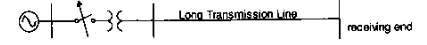
\includegraphics[width=0.8\textwidth]{Figs/Q39.png}
    \caption{}
    \label{fig:1.29}
\end{figure}
\begin{enumerate}
    \item The magnitude of terminal voltage decreases, and the field current does not change.
    \item The magnitude of terminal voltage increases, and the field current does not change.
    \item The magnitude of terminal voltage increases, and the field current increases.
    \item The magnitude of terminal voltage does not change, and the field current decreases.
\end{enumerate}
\hfill\brak{GATE \ EE \ 2010}

%Q.40
\item A separately excited dc machine is coupled to a 50 Hz, three-phase, 4-pole induction machine as shown in the figure. The dc machine is energized first and the machines rotate at 1600 rpm. Subsequently the induction machine is also connected to a 50 Hz, three-phase source, the phase sequence being consistent with the direction of rotation. In steady state,
\begin{figure}[H]
    \centering
    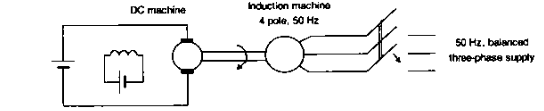
\includegraphics[width=0.9\textwidth]{Figs/Q40.png}
    \caption{}
    \label{fig:1.30}
\end{figure}
\begin{enumerate}
    \item both machines act as generators
    \item the dc machine acts as a generator, and the induction machine acts as a motor
    \item the dc machine acts as a motor, and the induction machine acts as a generator
    \item both machines act as motors
\end{enumerate}
\hfill\brak{GATE \ EE \ 2010}

%Q.41
\item A balanced star-connected and purely resistive load is connected at the secondary of a star-delta transformer as shown in the figure. The line-to-line voltage rating of the transformer is 110 V / 220 V. Neglecting the non-idealities of the transformer, the impedance `Z` of the equivalent star-connected load, referred to the primary side of the transformer, is:
\begin{figure}[H]
    \centering
    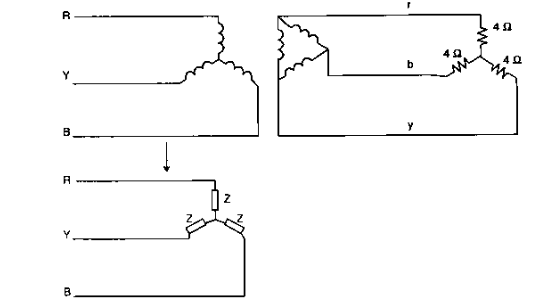
\includegraphics[width=0.9\textwidth]{Figs/Q41.png}
    \caption{}
    \label{fig:1.31}
\end{figure}
\begin{enumerate}
    \begin{multicols}{2}
        \item $\brak{3+j0}\Omega$
        \item $\brak{0.866-j0.5}\Omega$
        \item $\brak{0.866+j0.5}\Omega$
        \item $\brak{1+j0}\Omega$
    \end{multicols}
\end{enumerate}
\hfill\brak{GATE \ EE \ 2010}

%Q.42
\item Consider a three-phase, 50 Hz, 11 kV distribution system. Each of the conductors is suspended by an insulator string having two identical porcelain insulators. The self capacitance of the insulator is 5 times the shunt capacitance between the link and the ground, as shown in the figure. The voltage across the two insulators are
\begin{figure}[H]
    \centering
    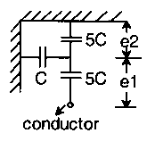
\includegraphics[width=0.3\textwidth]{Figs/Q42.png}
    \caption{}
    \label{fig:1.32}
\end{figure}
\begin{enumerate}
    \begin{multicols}{2}
        \item e1=3.74 kV, e2=2.61 kV
        \item e1=3.46 kV, e2=2.89 kV
        \item e1=6.0 kV, e2=4.23 kV
        \item e1=5.5 kV, e2=5.5 kV
    \end{multicols}
\end{enumerate}
\hfill\brak{GATE \ EE \ 2010}

%Q.43
\item Consider a three-core, three-phase, 50 Hz, 11 kV cable whose conductors are denoted as R, Y and B in the figure. The inter-phase capacitance \brak{C1} between each pair of conductors is 0.2 µF and the capacitance between each line conductor and the sheath is 0.4 µF. The per-phase charging current is
\begin{figure}[H]
    \centering
    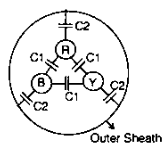
\includegraphics[width=0.4\textwidth]{Figs/Q43.png}
    \caption{}
    \label{fig:1.33}
\end{figure}
\begin{enumerate}
    \begin{multicols}{4}
        \item 2.0 A
        \item 2.4 A
        \item 2.7 A
        \item 3.5 A
    \end{multicols}
\end{enumerate}
\hfill\brak{GATE \ EE \ 2010}

%Q.44
\item For the power system shown in the figure below, the specifications of the components are the following:
G1: 25 kV, 100 MVA, $X=9\%$
G2: 25 kV, 100 MVA, $X=9\%$
T1: 25 kV/220 kV, 90 MVA, $X=12\%$
T2: 220 kV/25 kV, 90 MVA, $X=12\%$
Line 1: 220 kV, X=150 ohms
\begin{figure}[H]
    \centering
    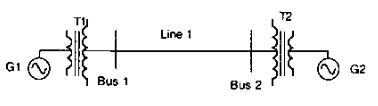
\includegraphics[width=0.6\textwidth]{Figs/Q44.png}
    \caption{}
    \label{fig:1.34}
\end{figure}
Choose 25 kV as the base voltage at the generator G1, and 200 MVA as the MVA base. The impedance diagram is
\begin{enumerate}
    \item \begin{figure}[H]\centering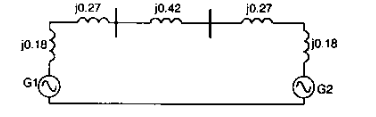
\includegraphics[width=0.8\textwidth]{Figs/Q44A.png}\caption{}\label{fig:1.35}\end{figure}
    \item \begin{figure}[H]\centering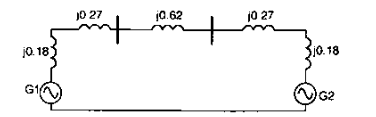
\includegraphics[width=0.8\textwidth]{Figs/Q44B.png}\caption{}\label{fig:1.36}\end{figure}
    \item \begin{figure}[H]\centering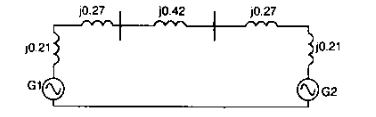
\includegraphics[width=0.8\textwidth]{Figs/Q44C.png}\caption{}\label{fig:1.37}\end{figure}
    \item \begin{figure}[H]\centering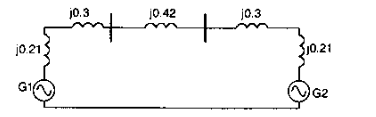
\includegraphics[width=0.8\textwidth]{Figs/Q44D.png}\caption{}\label{fig:1.38}\end{figure}
\end{enumerate}
\hfill\brak{GATE \ EE \ 2010}

%Q.45
\item The transistor circuit shown uses a silicon transistor with $V_{BE}=0.7 V$, $I_C \approx I_E$ and a dc current gain of 100. The value of $V_0$ is
\begin{figure}[H]
    \centering
    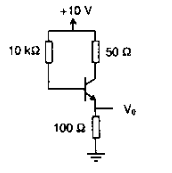
\includegraphics[width=0.3\textwidth]{Figs/Q45.png}
    \caption{}
    \label{fig:1.39}
\end{figure}
\begin{enumerate}
    \begin{multicols}{2}
        \item 4.65 V
        \item 5 V
        \item 6.3 V
        \item 7.23 V
    \end{multicols}
\end{enumerate}
\hfill\brak{GATE \ EE \ 2010}

%Q.46
\item The TTL circuit shown in the figure is fed with the waveform X \brak{also\ shown}. All gates have equal propagation delay of 10 ns. The output Y of the circuit is
\begin{figure}[H]
    \centering
    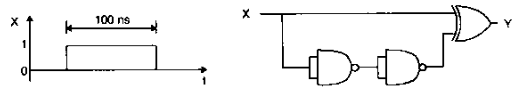
\includegraphics[width=0.7\textwidth]{Figs/Q46.png}
    \caption{}
    \label{fig:1.40}
\end{figure}
\begin{enumerate}
    \item \begin{figure}[H]\centering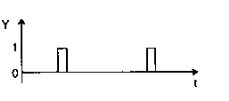
\includegraphics[width=0.6\textwidth]{Figs/Q46A.png}\caption{}\label{fig:1.41}\end{figure}
    \item \begin{figure}[H]\centering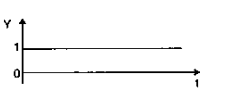
\includegraphics[width=0.6\textwidth]{Figs/Q46B.png}\caption{}\label{fig:1.42}\end{figure}
    \item \begin{figure}[H]\centering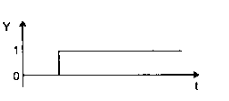
\includegraphics[width=0.6\textwidth]{Figs/Q46C.png}\caption{}\label{fig:1.43}\end{figure}
    \item \begin{figure}[H]\centering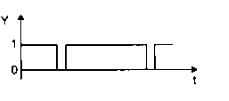
\includegraphics[width=0.6\textwidth]{Figs/Q46D.png}\caption{}\label{fig:1.44}\end{figure}
\end{enumerate}
\hfill\brak{GATE \ EE \ 2010}

%Q.47
\item When a "CALL Addr" instruction is executed, the CPU carries out the following sequential operations internally:
Note: \brak{R} means content of register R, \brak{\brak{R}} means content of memory location pointed to by R, PC means Program Counter, SP means Stack Pointer
\begin{enumerate}
    \item \brak{SP} incremented; $\brak{PC} \leftarrow Addr$; $\brak{\brak{SP}} \leftarrow \brak{PC}$
    \item $\brak{PC} \leftarrow Addr$; $\brak{\brak{SP}} \leftarrow \brak{PC}$; \brak{SP} incremented
    \item $\brak{PC} \leftarrow Addr$; \brak{SP} incremented; $\brak{\brak{SP}} \leftarrow \brak{PC}$
    \item $\brak{\brak{SP}} \leftarrow \brak{PC}$; \brak{SP} incremented; $\brak{PC} \leftarrow Addr$
\end{enumerate}
\hfill\brak{GATE \ EE \ 2010}

\newpage
\begin{flushleft}
\textbf{Common Data for Questions 48 and 49:}
\end{flushleft}
A separately excited DC motor runs at 1500 rpm under no-load with 200 V applied to the armature. The field voltage is maintained at its rated value. The speed of the motor, when it delivers a torque of 5 Nm, is 1400 rpm as shown in the figure. The rotational losses and armature reaction are neglected.
\begin{figure}[H]
    \centering
    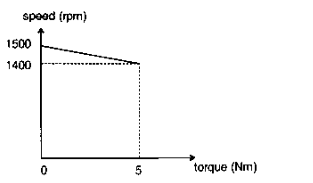
\includegraphics[width=0.5\textwidth]{Figs/Q48.png}
    \caption{}
    \label{fig:1.45}
\end{figure}

%Q.48
\item The armature resistance of the motor is
\begin{enumerate}
    \begin{multicols}{2}
        \item 2 $\Omega$
        \item 3.4 $\Omega$
        \item 4.4 $\Omega$
        \item 7.7 $\Omega$
    \end{multicols}
\end{enumerate}
\hfill\brak{GATE \ EE \ 2010}

%Q.49
\item For the motor to deliver a torque of 2.5 Nm at 1400 rpm, the armature voltage to be applied is
\begin{enumerate}
    \begin{multicols}{2}
        \item 125.5 V
        \item 193.3 V
        \item 200 V
        \item 241.7 V
    \end{multicols}
\end{enumerate}
\hfill\brak{GATE \ EE \ 2010}

\begin{flushleft}
\textbf{Common Data for Questions 50 and 51:}
\end{flushleft}
Given $f\brak{t}$ and $g\brak{t}$ as shown below:
\begin{figure}[H]
    \centering
    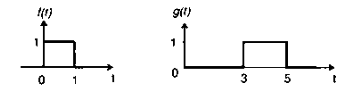
\includegraphics[width=0.6\textwidth]{Figs/Q50.png}
    \caption{}
    \label{fig:1.46}
\end{figure}

%Q.50
\item $g\brak{t}$ can be expressed as
\begin{enumerate}
    \begin{multicols}{2}
        \item $g\brak{t} = f\brak{2t-3}$
        \item $g\brak{t} = f\brak{\frac{t}{2}-3}$
        \item $g\brak{t} = f\brak{2t-\frac{3}{2}}$
        \item $g\brak{t} = f\brak{\frac{t}{2}-\frac{3}{2}}$
    \end{multicols}
\end{enumerate}
\hfill\brak{GATE \ EE \ 2010}

%Q.51
\item The Laplace transform of $g\brak{t}$ is
\begin{enumerate}
    \begin{multicols}{2}
        \item $\frac{1}{s}\brak{e^{3s}-e^{5s}}$
        \item $\frac{1}{s}\brak{e^{-3s}-e^{-5s}}$
        \item $\frac{e^{-3s}}{s}\brak{1-e^{-2s}}$
        \item $\frac{1}{s}\brak{e^{-5s}-e^{-3s}}$
    \end{multicols}
\end{enumerate}
\hfill\brak{GATE \ EE \ 2010}

\newpage
\begin{flushleft}
\textbf{Statement for Linked Answer Questions 52 and 53:}
\end{flushleft}
The following Karnaugh map represents a function F.
\begin{table}[H]
    \centering
    \begin{tabular}{l|c|c|c|c|}
      \multicolumn{1}{c}{F} & \multicolumn{4}{c}{YZ} \\
      \cline{2-5}
      & 00 & 01 & 11 & 10 \\
      \hline
      \multicolumn{1}{|l|}{X=0} & 1 & 1 & 1 & 0 \\
      \hline
      \multicolumn{1}{|l|}{X=1} & 0 & 0 & 1 & 0 \\
      \hline
    \end{tabular}
    \caption{}
    \label{table:1.1}
\end{table}

%Q.52
\item A minimized form of the function F is
\begin{enumerate}
    \begin{multicols}{2}
        \item $F=\overline{X}Y+YZ$
        \item $F=\overline{X}\overline{Y}+YZ$
        \item $F=\overline{X}\overline{Y}+Y\overline{Z}$
        \item $F=\overline{X}\overline{Y}+\overline{Y}Z$
    \end{multicols}
\end{enumerate}
\hfill\brak{GATE \ EE \ 2010}

%Q.53
\item Which of the following circuits is a realization of the above function F?
\begin{enumerate}
    \item \begin{figure}[H]\centering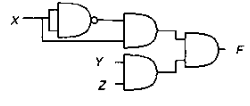
\includegraphics[width=0.7\textwidth]{Figs/Q53A.png}\caption{}\label{fig:1.47}\end{figure}
    \item \begin{figure}[H]\centering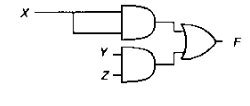
\includegraphics[width=0.7\textwidth]{Figs/Q53B.png}\caption{}\label{fig:1.48}\end{figure}
    \item \begin{figure}[H]\centering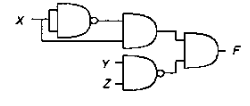
\includegraphics[width=0.7\textwidth]{Figs/Q53C.png}\caption{}\label{fig:1.49}\end{figure}
    \item \begin{figure}[H]\centering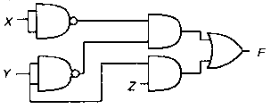
\includegraphics[width=0.7\textwidth]{Figs/Q53D.png}\caption{}\label{fig:1.50}\end{figure}
\end{enumerate}
\hfill\brak{GATE \ EE \ 2010}

\begin{flushleft}
\textbf{Statement for Linked Answer Questions 54 and 55:}
\end{flushleft}
The L-C circuit shown in the figure has an inductance $L=1$ mH and a capacitance $C=10 \mu F$.
\begin{figure}[H]
    \centering
    \includegraphics[width=0.4\textwidth]{Figs/Q54.png}
    \caption{}
    \label{fig:1.51}
\end{figure}

%Q.54
\item The initial current through the inductor is zero, while the initial capacitor voltage is 100 V. The switch is closed at $t=0$. The current i through the circuit is:
\begin{enumerate}
    \begin{multicols}{2}
        \item $5\cos\brak{5 \times 10^3 t}$ A
        \item $5\sin\brak{10^4 t}$ A
        \item $10\cos\brak{5 \times 10^3 t}$ A
        \item $10\sin\brak{10^4 t}$ A
    \end{multicols}
\end{enumerate}
\hfill\brak{GATE \ EE \ 2010}

%Q.55
\item The L-C circuit of Q54 is used to commutate a thyristor, which is initially carrying a current of 5 A as shown in the figure below. The values and initial conditions of L and C are the same as in Q54. The switch is closed at $t=0$. If the forward drop is negligible, the time taken for the device to turn off is
\begin{figure}[H]
    \centering
    \includegraphics[width=0.6\textwidth]{Figs/Q55.png}
    \caption{}
    \label{fig:1.52}
\end{figure}
\begin{enumerate}
    \begin{multicols}{4}
        \item 52 $\mu$s
        \item 156 $\mu$s
        \item 312 $\mu$s
        \item 26 $\mu$s
    \end{multicols}
\end{enumerate}
\hfill\brak{GATE \ EE \ 2010}
\newpage
\begin{flushleft}
\textbf{General Aptitude (GA) Questions}
\end{flushleft}

\textbf{Q.56 - Q.60 carry one mark each.}

%Q.56
\item 25 persons are in a room. 15 of them play hockey, 17 of them play football and 10 of them play both hockey and football. Then the number of persons playing neither hockey nor football is:
\begin{enumerate}
    \begin{multicols}{4}
        \item 2
        \item 17
        \item 13
        \item 3
    \end{multicols}
\end{enumerate}
\hfill\brak{GATE \ EE \ 2010}

%Q.57
\item Choose the most appropriate word from the options given below to complete the following sentence:
If we manage to \_\_\_\_\_\_\_ our natural resources, we would leave a better planet for our children.
\begin{enumerate}
    \begin{multicols}{2}
        \item uphold
        \item restrain
        \item cherish
        \item conserve
    \end{multicols}
\end{enumerate}
\hfill\brak{GATE \ EE \ 2010}

%Q.58
\item The question below consists of a pair of related words followed by four pairs of words. Select the pair that best expresses the relation in the original pair.
Unemployed: Worker
\begin{enumerate}
    \item fallow: land
    \item unaware: sleeper
    \item wit: jester
    \item renovated: house
\end{enumerate}
\hfill\brak{GATE \ EE \ 2010}

%Q.59
\item Which of the following options is the closest in meaning to the word below:
Circuitous
\begin{enumerate}
    \begin{multicols}{2}
        \item cyclic
        \item indirect
        \item confusing
        \item crooked
    \end{multicols}
\end{enumerate}
\hfill\brak{GATE \ EE \ 2010}

%Q.60
\item Choose the most appropriate word from the options given below to complete the following sentence:
His rather casual remarks on politics \_\_\_\_\_\_\_ his lack of seriousness about the subject.
\begin{enumerate}
    \begin{multicols}{2}
        \item masked
        \item belied
        \item betrayed
        \item suppressed
    \end{multicols}
\end{enumerate}
\hfill\brak{GATE \ EE \ 2010}

\textbf{Q.61 - Q.65 carry two marks each.}

%Q.61
\item Hari \brak{H}, Gita \brak{G}, Irfan \brak{I} and Saira \brak{S} are siblings \brak{i.e. brothers and sisters}. All were born on 1st January. The age difference between any two successive siblings \brak{that\ is\ born\ one\ after\ another} is less than 3 years. Given the following facts:
\begin{enumerate}
    \item[i.] Hari's age + Gita's age $>$ Irfan's age + Saira's age.
    \item[ii.] The age difference between Gita and Saira is 1 year. However, Gita is not the oldest and Saira is not the youngest.
    \item[iii.] There are no twins.
\end{enumerate}
In what order were they born \brak{oldest\ first}?
\begin{enumerate}
    \begin{multicols}{4}
        \item HSIG
        \item SGHI
        \item IGSH
        \item IHSG
    \end{multicols}
\end{enumerate}
\hfill\brak{GATE \ EE \ 2010}

%Q.62
\item 5 skilled workers can build a wall in 20 days; 8 semi-skilled workers can build a wall in 25 days; 10 unskilled workers can build a wall in 30 days. If a team has 2 skilled, 6 semi-skilled and 5 unskilled workers, how long will it take to build the wall?
\begin{enumerate}
    \begin{multicols}{4}
        \item 20 days
        \item 18 days
        \item 16 days
        \item 15 days
    \end{multicols}
\end{enumerate}
\hfill\brak{GATE \ EE \ 2010}

%Q.63
\item Modern warfare has changed from large scale clashes of armies to suppression of civilian populations. Chemical agents that do their work silently appear to be suited to such warfare; and regretfully, there exist people in military establishments who think that chemical agents are useful tools for their cause.
Which of the following statements best sums up the meaning of the above passage:
\begin{enumerate}
    \item Modern warfare has resulted in civil strife.
    \item Chemical agents are useful in modern warfare.
    \item Use of chemical agents in warfare would be undesirable.
    \item People in military establishments like to use chemical agents in war.
\end{enumerate}
\hfill\brak{GATE \ EE \ 2010}

%Q.64
\item Given digits 2, 2, 3, 3, 3, 4, 4, 4, 4 how many distinct 4 digit numbers greater than 3000 can be formed?
\begin{enumerate}
    \begin{multicols}{4}
        \item 50
        \item 51
        \item 52
        \item 54
    \end{multicols}
\end{enumerate}
\hfill\brak{GATE \ EE \ 2010}

%Q.65
\item If $137+276=435$ how much is $731+672$?
\begin{enumerate}
    \begin{multicols}{2}
        \item 534
        \item 1403
        \item 1623
        \item 1513
    \end{multicols}
\end{enumerate}
\hfill\brak{GATE \ EE \ 2010}

\end{enumerate}
\end{document}
\end{enumerate}
\end{document}
